\section{菲涅耳入射效应}\label{sec:菲涅耳入射效应}
图形学中许多BRDF模型都没有考虑到菲涅耳反射会减少到达多层物体底层光量的事实。
考虑一张抛光的木桌或者涂了光泽油漆的墙面:如果你正对着看向它们的表面,
你主要看到的是木头或油漆颜料的颜色。随着你把你的视角移向掠角,
你会看到更少的底色,因为它被随菲涅耳效应而增加的光泽反射淹没了。

本节中,我们将实现由\citet{AshikhminPhong,Ashikhmin01012000}
\sidenote{译者注:原文文献年份标注可能有误,已修正。}
开发的BRDF模型,它刻画了覆盖有光泽镜面表面的漫反射表面。
在考虑了菲涅耳效应后,来自漫反射曲面的的反射效应会由剩余能量量值调制。
\reffig{8.23}展示了该想法:当入射方向接近法线时,大部分光会透射到
漫反射层,漫反射项占主要部分。而当入射方向接近掠角时,主要反射模式则是光泽反射。
\reffig{12.19}的汽车模型就给它的车漆用的本模型。
\begin{lstlisting}
`\refcode{BxDF Declarations}{+=}\lastnext{BxDFDeclarations}`
class `\initvar{FresnelBlend}{}` : public `\refvar{BxDF}{}` {
public:
    `\refcode{FresnelBlend Public Methods}{}`
private:
    `\refcode{FresnelBlend Private Data}{}`
};
\end{lstlisting}

\begin{figure}[htbp]
    \centering
    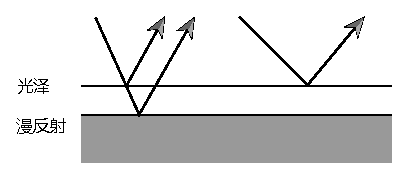
\includegraphics[width=0.65\linewidth]{Pictures/chap08/Fresnelincidence.eps}
    \caption{\refvar{FresnelBlend}{} BRDF刻画漫反射底层之上具有光泽层的曲面效果。
    随着向量${\bm\omega}_{\mathrm{i}}$和${\bm\omega}_{\mathrm{o}}$射入的角度移向掠角(右例),
    到达漫反射底层的光量因菲涅耳效应而减少,漫反射层变得更不明显了。}
    \label{fig:8.23}
\end{figure}

该模型接收两个光谱,一个表示漫反射和镜面反射,一个为光泽层的微面分布。
\begin{lstlisting}
`\refcode{BxDF Method Definitions}{+=}\lastnext{BxDFMethodDefinitions}`
`\refvar{FresnelBlend}{}`::`\refvar{FresnelBlend}{}`(const `\refvar{Spectrum}{}` &Rd, const `\refvar{Spectrum}{}` &Rs,
                           `\refvar{MicrofacetDistribution}{}` *distribution) 
    : `\refvar{BxDF}{}`(`\refvar{BxDFType}{}`(`\refvar[BSDFREFLECTION]{BSDF\_REFLECTION}{}` | `\refvar[BSDFGLOSSY]{BSDF\_GLOSSY}{}`)),
      `\refvar[FresnelBlend::Rd]{Rd}{}`(Rd), `\refvar[FresnelBlend::Rs]{Rs}{}`(Rs), `\refvar[FresnelBlend::distribution]{distribution}{}`(distribution) { }
\end{lstlisting}
\begin{lstlisting}
`\initcode{FresnelBlend Private Data}{=}`
const `\refvar{Spectrum}{}` `\initvar[FresnelBlend::Rd]{Rd}{}`, `\initvar[FresnelBlend::Rs]{Rs}{}`;
`\refvar{MicrofacetDistribution}{}` *`\initvar[FresnelBlend::distribution]{distribution}{}`;
\end{lstlisting}

该模型基于光泽镜面项和漫反射项的加权和。考虑到互易性和能量守恒,推导出光泽镜面项为
\sidenote{译者注:原文漏写了$F_{\mathrm{r}}$的下标,已修正。}
\begin{align*}
    f_{\mathrm{r}}({\bm p},{\bm\omega}_{\mathrm{o}},{\bm\omega}_{\mathrm{i}})
    =\frac{D({\bm\omega}_{\mathrm{h}})F_{\mathrm{r}}({\bm\omega}_{\mathrm{o}})}
    {4({\bm\omega}_{\mathrm{h}}\cdot{\bm\omega}_{\mathrm{i}})
    (\max(({\bm n}\cdot{\bm\omega}_{\mathrm{o}}),({\bm n}\cdot{\bm\omega}_{\mathrm{i}})))}\, ,
\end{align*}
其中$D({\bm\omega}_{\mathrm{h}})$是微面分布项,$F_{\mathrm{r}}({\bm\omega}_{\mathrm{o}})$表示
菲涅耳反射率。注意它和Torrance-Sparrow模型非常像。
\citeauthor{AshikhminPhong}的模型的关键是推导出仍然遵循互易性和
能量守恒的漫反射项。其推导依赖于\citet{Schlick1993}给出的对菲涅耳反射方程的近似,即
\sidenote{译者注:原文以$\theta$来表示代入的角度变量,但可能引起歧义,
实际上该论文代入的角度是半角大小$\theta_{\mathrm{h}}$,译文已修改。}
\begin{align*}
    F_{\mathrm{r}}(\cos\theta_{\mathrm{h}})=R+(1-R)(1-\cos\theta_{\mathrm{h}})^5\, ,
\end{align*}
其中$R$是按法线入射时的曲面反射率。

有了该菲涅耳项,下式的漫反射项就能以物理上较合理的方式成功刻画基于菲涅耳衰减的漫反射。
\begin{align*}
    f_{\mathrm{r}}({\bm p},{\bm\omega}_{\mathrm{o}},{\bm\omega}_{\mathrm{i}})
    =\frac{28R_{\mathrm{d}}}{23\pi}(1-R_{\mathrm{s}})
    \left(1-\left(1-\frac{1}{2}({\bm n}\cdot{\bm\omega}_{\mathrm{i}})\right)^5\right)
    \left(1-\left(1-\frac{1}{2}({\bm n}\cdot{\bm\omega}_{\mathrm{o}})\right)^5\right)\, .
\end{align*}

我们不会在这里引入对该结果的推导。
\begin{lstlisting}
`\initcode{FresnelBlend Public Methods}{=}`
`\refvar{Spectrum}{}` `\initvar{SchlickFresnel}{}`(`\refvar{Float}{}` cosTheta) const {
    auto pow5 = [](`\refvar{Float}{}` v) { return (v * v) * (v * v) * v; };
    return `\refvar[FresnelBlend::Rs]{Rs}{}` + pow5(1 - cosTheta) * (`\refvar{Spectrum}{}`(1.) - `\refvar[FresnelBlend::Rs]{Rs}{}`);
}
\end{lstlisting}
\begin{lstlisting}
`\refcode{BxDF Method Definitions}{+=}\lastnext{BxDFMethodDefinitions}`
`\refvar{Spectrum}{}` `\refvar{FresnelBlend}{}`::`\initvar[FresnelBlend::f]{f}{}`(const `\refvar{Vector3f}{}` &wo, const `\refvar{Vector3f}{}` &wi) const {
    auto pow5 = [](`\refvar{Float}{}` v) { return (v * v) * (v * v) * v; };
    `\refvar{Spectrum}{}` diffuse = (28.f/(23.f*`\refvar{Pi}{}`)) * `\refvar[FresnelBlend::Rd]{Rd}{}` *
        (`\refvar{Spectrum}{}`(1.f) - `\refvar[FresnelBlend::Rs]{Rs}{}`) * 
        (1 - pow5(1 - .5f * `\refvar{AbsCosTheta}{}`(wi))) *
        (1 - pow5(1 - .5f * `\refvar{AbsCosTheta}{}`(wo)));
    `\refvar{Vector3f}{}` wh = wi + wo;
    if (wh.x == 0 && wh.y == 0 && wh.z == 0) return `\refvar{Spectrum}{}`(0);
    wh = `\refvar{Normalize}{}`(wh);
    `\refvar{Spectrum}{}` specular = `\refvar[FresnelBlend::distribution]{distribution}{}`->`\refvar[MicrofacetDistribution::D]{D}{}`(wh) /
        (4 * `\refvar{AbsDot}{}`(wi, wh) *
         std::max(`\refvar{AbsCosTheta}{}`(wi), `\refvar{AbsCosTheta}{}`(wo))) *
         `\refvar{SchlickFresnel}{}`(`\refvar{Dot}{}`(wi, wh));
    return diffuse + specular;
}
\end{lstlisting}
